\chapter{Marco Aplicativo}


\section{Descripción general de la solución} 
\setlength{\parskip}{5mm}
\setlength{\parskip}{0mm}

\newpage

\section{Aplicación de la metodología Scrum}

A continuación, en la siguiente Tabla se muestran las actividades programadas para los Sprint en pro del desarrollo del sistema. 
\subsection{Lista de Objetivos (Pila del Producto)}

\begin{table}[H]	
\begin{center}
\begin{tabular}{ | m{2cm} | m{9cm}| m{3cm}| } 
 \hline
 Sprint & Actividad & Fecha \\
 \hline
 1. 
 & 
 \begin{itemize}
 	\item Instalación de las herramientas de desarrollo necesarias.
 	\item Configuración de los ambientes de desarrollo.
 	\item Maquetado de las Interfaces
 	\item Elaboración del Diagrama de Modelo relacional para la base de datos.
 \end{itemize}
 & 
 01/02/2017 - 14/02/2017\\
 \hline

 2. 
 & 
 \begin{itemize}
 	\item Desarrollo del modulo de registro.
 	\item Realización de pruebas de funcionalidad.
 \end{itemize}
 & 
 15/02/2017 - 28/02/2017\\
 \hline

 3.
 & 
 \begin{itemize}
 	\item Desarrollo de la funcionalidad de recuperar contraseña
 	\item Desarrollo del modulo de gestión de solicitudes
 	\item Desarrollo de la funcionalidad de solicitar inspección
 	\item Realización de pruebas de funcionalidad
 \end{itemize}
 & 
 01/03/2017 - 15/03/2017\\
 \hline
 

 


\end{tabular}
\caption{Pila del Producto. Fuente: El Autor.}
\label{Tabla:15}
\end{center}
\end{table}	

\newpage

\begin{table}[H]	
\begin{center}
\begin{tabular}{ | m{2cm} | m{9cm}| m{3cm}| } 
 \hline
 Sprint & Actividad & Fecha \\
 \hline
 4.
 & 
 \begin{itemize}
 	\item Desarrollo de la funcionalidad de gestión de tickets de solicitudes de inspección
 	\item Desarrollo de la funcionalidad de consultar solicitudes de inspección
 	\item Realización de pruebas de funcionalidad
 \end{itemize}
 & 
 16/03/2017 - 31/03/2017\\
 \hline
  5. 
 & 
 \begin{itemize}
 	\item Desarrollo de la funcionalidad de realizar inspección
 	\item Desarrollo de la funcionalidad de gestionar inspección
 	\item Desarrollo de la funcionalidad de generación de pdf
 	\item Realización de pruebas de funcionalidad
 \end{itemize}
 & 
 01/04/2017 - 15/04/2017\\
 \hline
6. 
 & 
 \begin{itemize}
 	\item Desarrollo del modulo administrativo
 	\item Desarrollo de la funcionalidad de Gestión de Usuarios (Taquilla Inspectores)
 	\item Realización de pruebas de funcionalidad
 \end{itemize}
 & 
 16/04/2017 - 30/04/2017\\
 \hline

 7. 
 & 
 \begin{itemize}
 	\item Desarrollo de la funcionalidad de Gestión de Titulares de Vehículo
 	\item Desarrollo de la funcionalidad de Gestión de Personas que trajeron el Vehículo a la inspección
 	\item Realización de pruebas de funcionalidad
 \end{itemize}
 & 
 01/05/2017 - 15/05/2017\\
 \hline

 8.
 & 
 \begin{itemize}
 	\item Desarrollo del Vehículo en formato SVG
 	\item Realización de pruebas de funcionalidad
 \end{itemize}
 &
 16/05/2017 - 30/05/2017\\
 \hline

\end{tabular}
\caption{Pila del Producto. Fuente: El Autor.}
\label{Tabla:15}
\end{center}
\end{table}	





\subsection{Lista de tareas de la iteración (Pila del Sprint)}
\setlength{\parskip}{5mm}

\textbf{-Sprint 1}: Se comenzó con la instalación de las herramientas necesarias para el desarrollo de la aplicación, las cuales fueron Python 2.7.9, PostgreSQL 9.4.3 y Django 1.10. 

Además se realizó el diseño y maquetado de la aplicación, a partir de los componente provistos por el Framework Bootstrap 4 y HMTL5 como base para el desarrollo de las interfaces de usuario. También se realizo el modelado de la base de datos en conjunto con los diagramas asociados al sistema. Finalmente se instalaron todas las dependencias necesarias en un ambiente virtual para la realización del sistema.


\textbf{-Sprint 2}: En este Sprint se desarrollaron parte de las funcionalidades pertinentes al modulo de registro, con sus validaciones respectivas para el correcto funcionamiento del sistema de registro. Luego se realización las pruebas de funcionalidad correspondientes para validar el funcionamiento esperado del sistema.

\textbf{-Sprint 3}: En este Sprint se terminaron de desarrollar las funcionalidades restantes del modulo de registro, se empezó el desarrollo del modulo de gestión de solicitudes, en el cual se implementaron parte de las funcionalidades tales como el solicitar una inspección. Además se realizaron las pruebas pertinentes para el correcto funcionamiento de la aplicación.

\textbf{-Sprint 4}: Se realizaron las funcionalidades de gestión de tickets de solicitud de inspección y consultar solicitudes de inspección, en esta ultima se obtuvieron las especificaciones de los campos por los cuales se filtrarían dichas solicitudes. Luego se realizaron las pruebas necesarias para validar el correcto funcionamiento de las funcionalidades desarrolladas.

\textbf{-Sprint 5}: En este Sprint se desarrollaron las funcionalidades de realizar inspección y la gestión de las mismas, además de la generación de la planilla en la cual se registran todos los datos de las especificaciones del vehículo e información relevante de la inspección. Se realizaron las pruebas funcionales para validar el correcto funcionamiento.

\textbf{-Sprint 6}: En este Sprint se desarrollo parte del modulo de administración, en especifico la funcionalidad de gestión de usuarios que comprende en editar, inactiva y eliminar usuarios. Además se realizaron las pruebas pertinentes para garantizar la correcta funcionalidad.

\textbf{-Sprint 7}: Se desarrollaron las funcionalidades restantes del modulo de administración, gestión de los titulares del vehículo y de las personas que trajeron el vehículo a inspeccionar. Seguidamente se realizaron las pruebas funcionales para validar un correcto funcionamiento.

\textbf{-Sprint 8}: Se desarrollo la imagen del carro en formato SVG y se validaron las partes pertinente para que cambiaran de color dependiendo del estado del vehículo. Se realizaron las pruebas correspondientes para finalizar la planilla de inspección.

\setlength{\parskip}{0mm}


\section{Requerimientos del Sistema } 
\setlength{\parskip}{5mm}
	De acuerdo a los requerimientos definidos por el cliente (Product Owner), se estableció las siguiente clasificación:

	\textbf{-Requerimientos Funcionales}: 

	\begin{itemize}
		\item Registro de usuarios por roles.
		\item Recuperar contraseña.
		\item Edición del perfil de usuario.
		\item Administración de los usuarios del sistema.
		\item Administración de los clientes del sistema (Titular, Persona que trajo el Vehículo).
		\item Creación de tickets para la inspección del vehículo.
		\item Consultar tickets creados.
		\item Consultar solicitudes de inspección.
		\item Registro de los datos de la inspección del vehículo.
		\item Gestionar solicitudes de inspección.
		\item Creación de una imagen de carro donde se muestren diferentes colores, para las partes del carro, dependiendo su estado.
	\end{itemize}

	\textbf{-Requerimientos no Funcionales}: 

	\begin{itemize}
		\item Validar las entradas de los datos para el correcto funcionamiento del sistema.
	\end{itemize}

\setlength{\parskip}{0mm}


\section{Perfiles de Usuario} 
\setlength{\parskip}{5mm}

\textbf{-Administrador}: Es el usuario encargado de gestionar tanto usuarios como a los clientes y propietarios de los vehículos inspeccionados.
	\begin{itemize}
		\item Búsqueda de usuarios del sistema.
		\item Búsqueda de titulares de los vehículos.
		\item Búsqueda de personas trajeron el vehículo a revisión. 
		\item Edición de titulares de vehículos.
		\item Edición de personas trajeron el vehículo a revisión.
		\item Edición y desactivación de usuarios Inspectores.
		\item Edición y desactivación de usuarios Taquilla.
		\item Reinicio de usuarios enviado les nuevas contraseñas.
	\end{itemize}

\textbf{-Inspector}: Este usuario puede crear una cuenta en el sistema para gestionar solicitudes de inspección de vehículo. También puede editar la información de su cuenta, ver la información de las solicitudes cerradas. 
	\begin{itemize}
		\item Creación y edición de una cuenta con su información básica para el uso del sistema.
		\item Visualización de las solicitudes de inspección pendientes por realizar.
		\item Vaciado de la información de la inspección del vehículo en el sistema.
		\item Gestión de la solicitud de inspección (verificación y guardado). 
		\item Visualizar información de las solicitudes de inspección.
		\item Búsqueda de solicitudes de inspección realizadas.
	\end{itemize}

\textbf{-Taquilla}: Este usuario puede crear una cuenta en el sistema para gestionar los tickets de atención, de las persona que requieran realizar una inspección.
	\begin{itemize}
		\item Creación y edición de una cuenta con su información básica para el uso del sistema.
		\item Creación de ticket para solicitud de inspección.
		\item Cancelar un ticket abierto de una solicitud de inspección 
		\item Búsqueda de tickets abiertos
	\end{itemize}


\setlength{\parskip}{0mm}


\section{Descripción del flujo asociado a la solución} 
\setlength{\parskip}{5mm}
\setlength{\parskip}{0mm}

\subsection{Proceso de creación de solicitud}
\setlength{\parskip}{5mm}
\setlength{\parskip}{0mm}

\subsection{Proceso de llenado de planilla de inspección}
\setlength{\parskip}{5mm}
\setlength{\parskip}{0mm}

\subsection{Proceso de gestión de solicitud de inspección}
\setlength{\parskip}{5mm}
\setlength{\parskip}{0mm}


\section{Análisis del modelo de datos y definición} 
\setlength{\parskip}{5mm}

En la elaboracion del modelo de datos pertenecientes a la aplicacion se crearon un total de veintiocho (28) tablas.

\setlength{\parskip}{0mm}

\subsection{Listado de tablas de la aplicación}

\setlength{\parskip}{5mm}

A continuación se presenta un listado con todas las tablas de la base de datos perteneciente al sistema desarrollado, junto con una breve descripción para cada una:


\textbf{-registro\_status}: Permite clasificar el estado del usuario (Activo,Inactivo).

\textbf{-registro\_tipousuario}: Permite clasificar a los usuarios por tipo (Administrador, Cliente, Taquilla).

\textbf{-registro\_usuario}: Permite almacenar los usuarios en el sistema.

\textbf{-rcs\_accesoriosbase}: Permite almacenar los accesorios básicos de la planilla.

\textbf{-rcs\_accesoriosvehiculo}: Tabla utilizada para representar los accesorios base de un vehículo.

\textbf{-rcs\_condicionesgeneralesbase}: Permite almacenar las condiciones generales básicas de la planilla.

\textbf{-rcs\_condicionesgeneralesvehiculo}: Tabla utilizada para representar las condiciones generales base de un vehículo.

\textbf{-rcs\_detallesdatos}: Permite almacenar lo detalles y datos de la planilla.

\textbf{-rcs\_documentospresentados}: Permite almacenar los documentos presentados básicos de la planilla.

\textbf{-rcs\_documentospresentadosbase}: Tabla utilizada para representar los documentos presentados base de un vehículo.

\textbf{-rcs\_estadosolicitud}: Permite almacenar los diferentes estado que puede poseer la planilla (Abierta, Por Revisar,Cerrada).

\textbf{-rcs\_estadovehiculo}: Permite almacenar los diferentes estado que puede poseer las partes del vehículo (Bueno, Regular,Malo).

\textbf{-rcs\_mecanicabase}: Permite almacenar las mecánicas básicas de la planilla.

\textbf{-rcs\_mecanicavehiculo}: Tabla utilizada para representar las mecánicas base de un vehículo.

\textbf{-rcs\_motivosolicitud}: Permite almacenar los diferentes motivos por lo cual se realiza la solicitud de inspección.

\textbf{-rcs\_solicitudinspeccion}: Permite almacenar las solicitudes de inspección realizadas por el sistema.

\textbf{-rcs\_tipomanejo}: Permite almacenar los diferentes tipos de manejo (Automático, Sincrónico).

\textbf{-rcs\_tipovehiculo}: Permite guardar la información de los diferentes tipos de vehículos (Sedan, Carga, Coupe)

\textbf{-rcs\_titularvehiculo}: Permite almacenar la información referente a los titulares de los vehículos.

\textbf{-rcs\_trajovehiculo}: Permite almacenar la información de las personas que trajeron el vehículo a inspección en lugar del titular del titular.

\textbf{-rcs\_vehiculo}: Permite almacenar la información referente al vehículo.

\textbf{-rcs\_vehiculo\_accesorios\_vehiculo}: Tabla utilizada para representar las relaciones ManyToMany de rcs\_accesoriosvehiculo y vehículo.

\textbf{-rcs\_vehiculo\_condiciones\_generales\_vehiculo}: Tabla utilizada para representar las relaciones ManyToMany de rcs\_condicionesgeneralesvehiculo y vehículo.

\textbf{-rcs\_vehiculo\_detalles\_datos}: Tabla utilizada para representar las relaciones ManyToMany de rcs\_detallesdatos y vehículo.

\textbf{-rcs\_vehiculo\_documentos\_presentados}: Tabla utilizada para representar las relaciones ManyToMany de rcs\_documentospresentados y vehículo.

\textbf{-rcs\_vehiculo\_mecanica\_vehiculo}: Tabla utilizada para representar las relaciones ManyToMany de rcs\_mecanicavehiculo y vehículo.

\textbf{-django\_migrations}: Permite almacenar y llevar un control de las migraciones aplicadas para cambiar la base de datos a lo largo del proceso de desarrollo.

\textbf{-django\_session}: Permite almacenar todos los valores usados en la sesión de los usuarios dentro de la aplicación.


\setlength{\parskip}{0mm}





\subsection{Modelo de datos}
\setlength{\parskip}{5mm}
\setlength{\parskip}{0mm}


\section{Servicios web maybe} 
\setlength{\parskip}{5mm}
\setlength{\parskip}{0mm}

\section{Descripción de los módulos del sistema y sus interfaces } 
\setlength{\parskip}{5mm}
El sistema web se encuentra divido en varios módulos. Los cuales están representados en la siguiente Figura.
\setlength{\parskip}{0mm}
\begin{figure}[H]
\begin{center}
	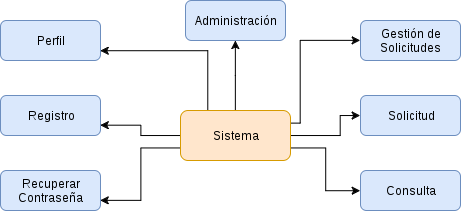
\includegraphics[width=\textwidth]{img/modulos_del_sistema.png}
\end{center}
\caption{Diagrama de módulos del sistema. Fuente:El Autor.}
\label{fig:Modulos_del_sistema}
\end{figure}


\textbf{Módulos}:
\begin{itemize}
	\item Administración: En este modulo el usuario con perfil administrador puede configurar parámetros referentes a los usuarios del sistema.
	
	\item Registro: En este modulo los usuarios pueden registrarse en este sistema ya sea como usuario tipo Inspectores o Taquilla.
	
	\item Perfil: Este modulo le permite al usuario modificar su información de contacto registrada en el sistema.
	
	\item Recuperar Contraseña: En este modulo los usuarios pueden recuperar su contraseña en caso de olvidarla. 
	
	\item Consulta: Este modulo hace énfasis en los filtros necesarios para la búsqueda de información dentro del sistema ya sea de solicitudes, usuarios o clientes (Aquellos que trajeron el carro a inspección)
	
	\item Solicitud: En este modulo los tipo de usuario Taquilla, al recibir un cliente, crean una solicitud de inspección.
	
	\item Gestión de Solicitudes: En este modulo los tipo de usuario Inspector realizan el registro de los datos de la inspección del vehículo y la gestión de las solicitudes de inspección.
	

\end{itemize}

\newpage
\subsection{Interfaces de la aplicación}
\setlength{\parskip}{5mm}

\textbf{-Interfaz de inicio de sesión}: La figura a continuación muestra el formulario de inicio de sesión para aquellos usuarios registrados en el sistema.

\begin{figure}[H]
\begin{center}
	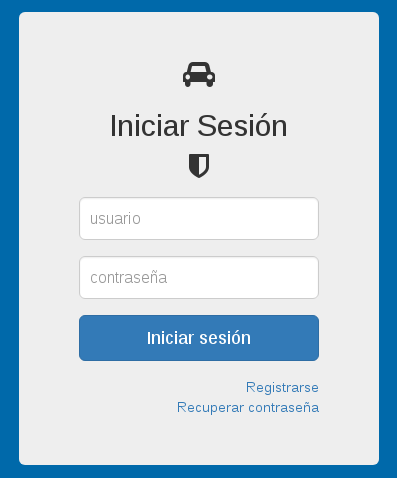
\includegraphics[width=8cm,height=10cm]{img/interfaces/inicio_sesion.png}
\end{center}
\caption{Interfaz de Inicio de Sesión. Fuente:Print Screen.}
\label{fig:interfaz_inicion_sesion}
\end{figure}

A partir de esta interfaz los usuarios registrados en el sistema podrán loguearse con su usuario y contraseña, en caso de no estar registrados se presenta la opción para registrarse, además se muestra la opción de recuperar contraseña en caso de que el usuario la haya olvidado
\newpage
\textbf{-Interfaz de recuperar contraseña}: La figura a continuación muestra el formulario de recuperación de contraseña para aquellos usuarios registrados en el sistema.


\begin{figure}[H]
\begin{center}
	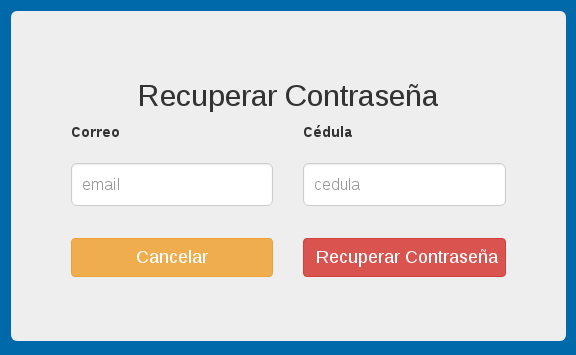
\includegraphics[width=14cm,height=6cm]{img/interfaces/recuperar_contrasena.png}
\end{center}
\caption{Interfaz de Recuperar Contraseña. Fuente: Print Screen.}
\label{fig:interfaz_recuperar_contrasena}
\end{figure}

A partir de esta interfaz los usuarios registrados en el sistema podrán recuperar su contraseña mediante el formulario incluyendo su correo y cédula. Se generara una contraseña aleatoria que sera enviada a su correo con la cual podrán acceder al sistema, para luego cambiar su contraseña a una propia.


\textbf{-Interfaz registro de usuarios}: La figura a continuación muestra el formulario de registro de usuarios para aquellos usuarios no registrados en el sistema.

\begin{figure}[H]
\begin{center}
	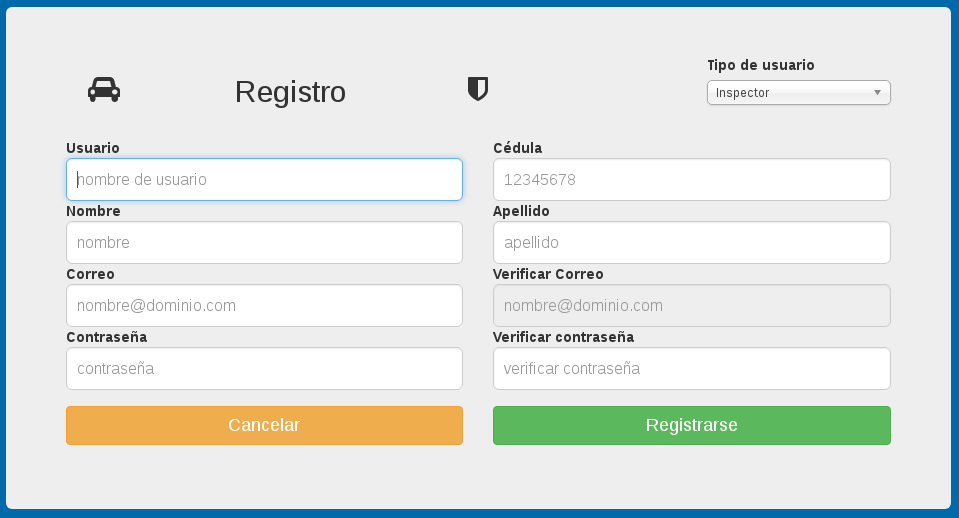
\includegraphics[width=14cm,height=6cm]{img/interfaces/registro_usuario.png}
\end{center}
\caption{Interfaz de Registro de Usuarios. Fuente: Print Screen.}
\label{fig:interfaz_registro_usuario}
\end{figure}

En esta interfaz los usuarios pueden registrarse bien sea como Inspectores o como usuarios Taquilla, ingresando su información personal.

\textbf{-Interfaz Configuración de Perfil}: La figura a continuación muestra el formulario de registro de usuarios para aquellos usuarios no registrados en el sistema.

\begin{figure}[H]
\begin{center}
	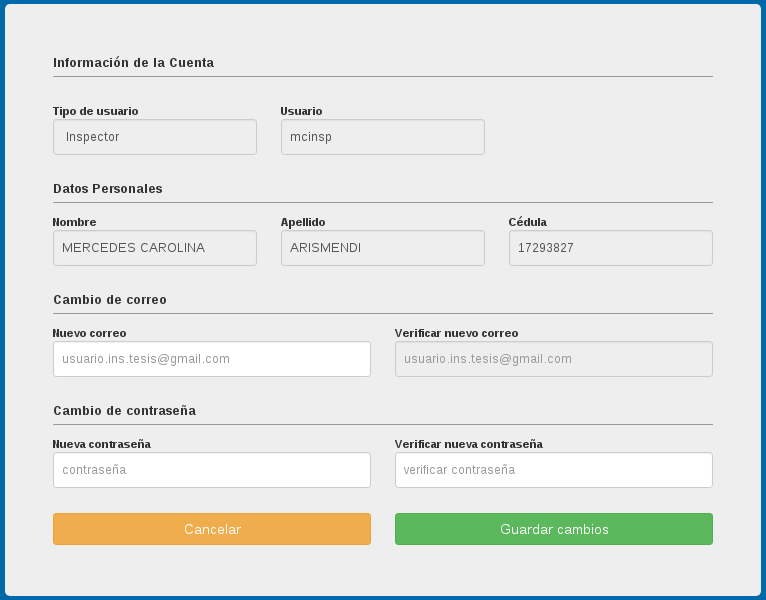
\includegraphics[width=12cm,height=8cm]{img/interfaces/editar_usuario.png}
\end{center}
\caption{Interfaz de Configuración del Perfil de Usuario. Fuente: Print Screen.}
\label{fig:interfaz_configuracion_usuario}
\end{figure}

En esta interfaz los usuarios pueden modificar su información personal ya sea el correo o contraseña.
\newpage

\textbf{-Interfaz Administrador bandeja de Usuarios}: La figura a continuación muestra el filtro y bandeja de los usuarios registrados en el sistema.

\begin{figure}[H]
\begin{center}
	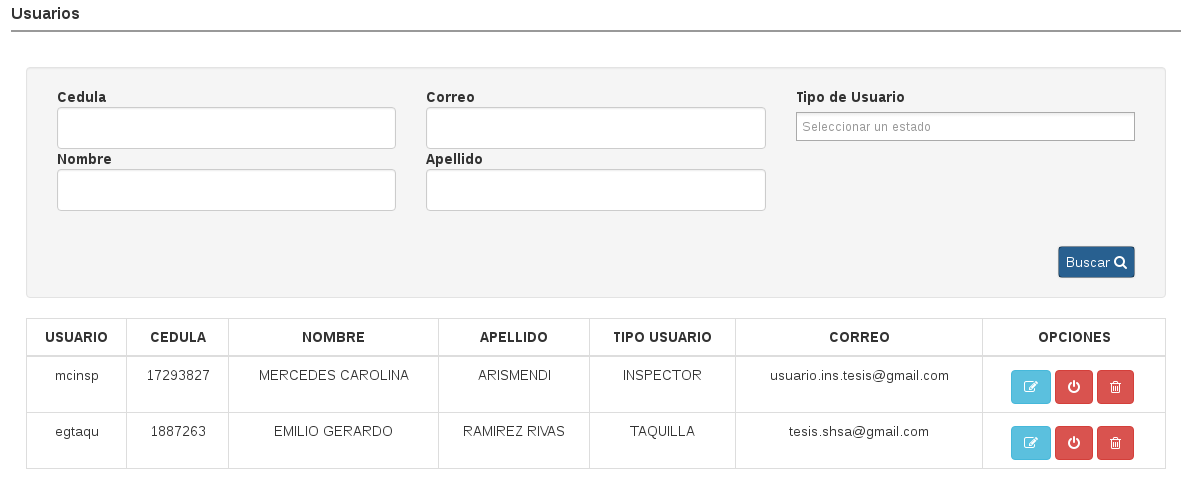
\includegraphics[width=\textwidth,height=7cm]{img/interfaces/bandeja_edicion_usuarios.png}
\end{center}
\caption{Interfaz de bandeja edición usuario por Administrador. Fuente: Print Screen.}
\label{fig:interfaz_bandeja_edicion_usuario}
\end{figure}

En esta interfaz los usuarios pueden ser modificados, inactivados y eliminados. Inactivados siempre y cuando no tengan una solicitud de inspección en proceso y eliminado siempre y cuando no tengan ninguna solicitud asociada al mismo.



\textbf{-Modal Inactivar Usuario}: La figura a continuación muestra el modal de confirmación para inactivar un usuario.

\begin{figure}[H]
\begin{center}
	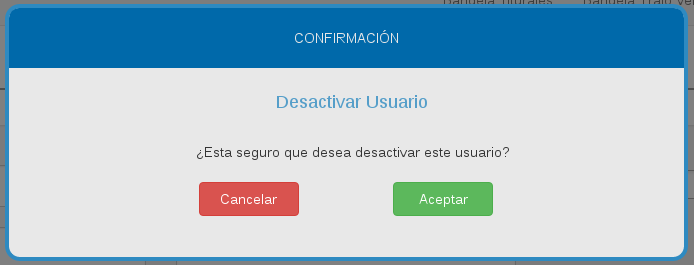
\includegraphics[width=14cm,height=6cm]{img/interfaces/modal_inactivar_usuario.png}
\end{center}
\caption{Modal Inactivar Usuario. Fuente: Print Screen.}
\label{fig:modal_confirmacion_inactivar_usuario}
\end{figure}

\textbf{-Modal Eliminar Usuario }: La figura a continuación muestra el modal de confirmación para eliminar un usuario.

\begin{figure}[H]
\begin{center}
	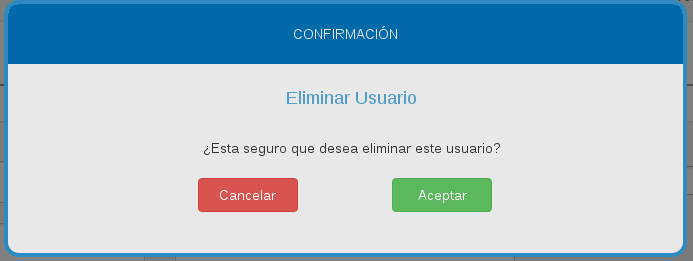
\includegraphics[width=14cm,height=6cm]{img/interfaces/modal_eliminar_usuario.png}
\end{center}
\caption{Modal Eliminar Usuario. Fuente: Print Screen.}
\label{fig:modal_confirmacion_eliminar_usuario}
\end{figure}


\textbf{-Interfaz Administrador Edición de Usuarios}: La figura a continuación muestra el formulario de edición de usuario por parte del administrador.

\begin{figure}[H]
\begin{center}
	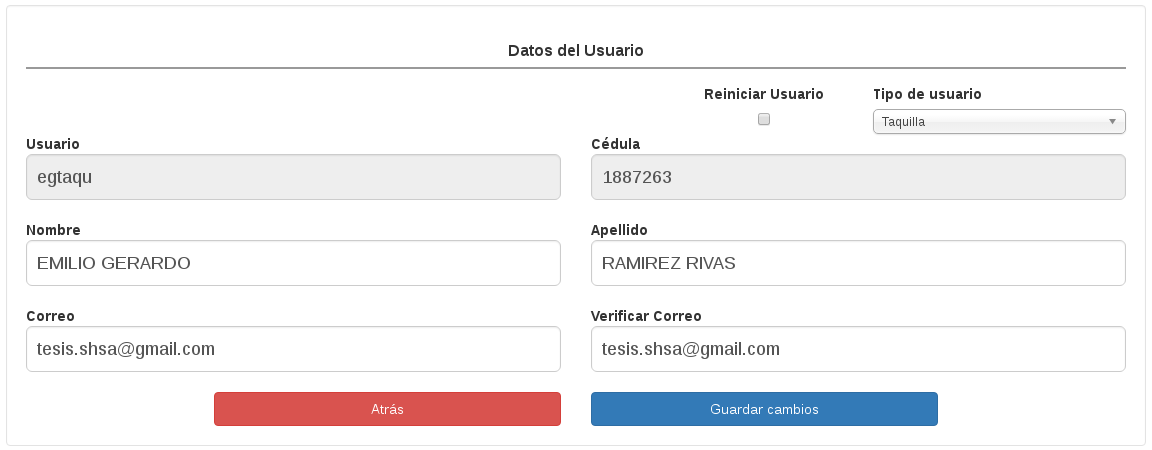
\includegraphics[width=\textwidth,height=6cm]{img/interfaces/editar_usuario_admin.png}
\end{center}
\caption{Interfaz de edición de usuario por Administrador. Fuente: Print Screen.}
\label{fig:interfaz_edicion_usuario_administrador}
\end{figure}

En esta interfaz el administrador puede cambiar tanto el nombre como el correo, el nombre no puede ser cambiado si el inspector ya proceso alguna solicitud. Además esta la función de reiniciar el usuario, el cual funciona como el recuperar contraseña en caso de que el usuario haya olvidado su correo o usuario registrado.


\textbf{-Interfaz creación de solicitud de inspección}: La figura a continuación muestra el formulario para la creación de una solicitud de inspección.

\begin{figure}[H]
\begin{center}
	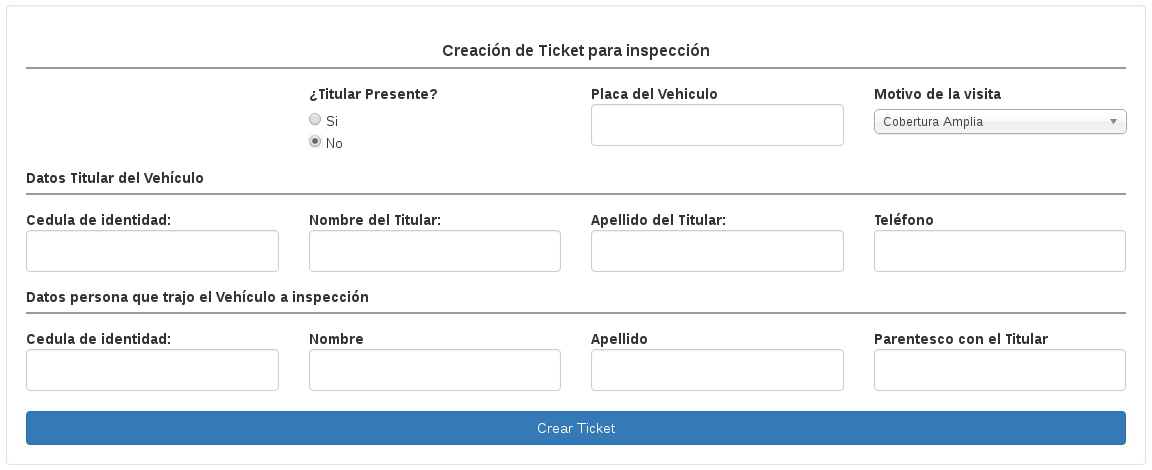
\includegraphics[width=\textwidth,height=7cm]{img/interfaces/crear_ticket_solicitud.png}
\end{center}
\caption{Interfaz de creación de solicitud de inspección. Fuente: Print Screen.}
\label{fig:interfaz_crear_solicitud_inspeccion}
\end{figure}

En esta interfaz el usuario Taquilla puede crear una solicitud de inspección con los datos del cliente, en caso de que el cliente exista, se llenan automáticamente al incluir la cédula. En caso de que no este el Titular se incluyen también los datos de la persona que trajo el vehículo a inspección.

\newpage
\textbf{-Modal crear solicitud de inspección }: La figura a continuación muestra el modal de confirmación para crear una solicitud de inspección.

\begin{figure}[H]
\begin{center}
	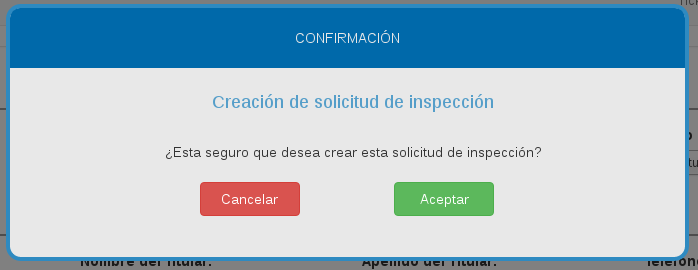
\includegraphics[width=14cm,height=6cm]{img/interfaces/modal_confirmar_creacion_solicitud.png}
\end{center}
\caption{Modal crear solicitud de inspección. Fuente: Print Screen.}
\label{fig:modal_confirmacion_crear_solicitud}
\end{figure}



\textbf{-Interfaz Taquilla bandeja de solicitudes}: La figura a continuación muestra el filtro y bandeja de las solicitudes de inspección creadas recientemente.

\begin{figure}[H]
\begin{center}
	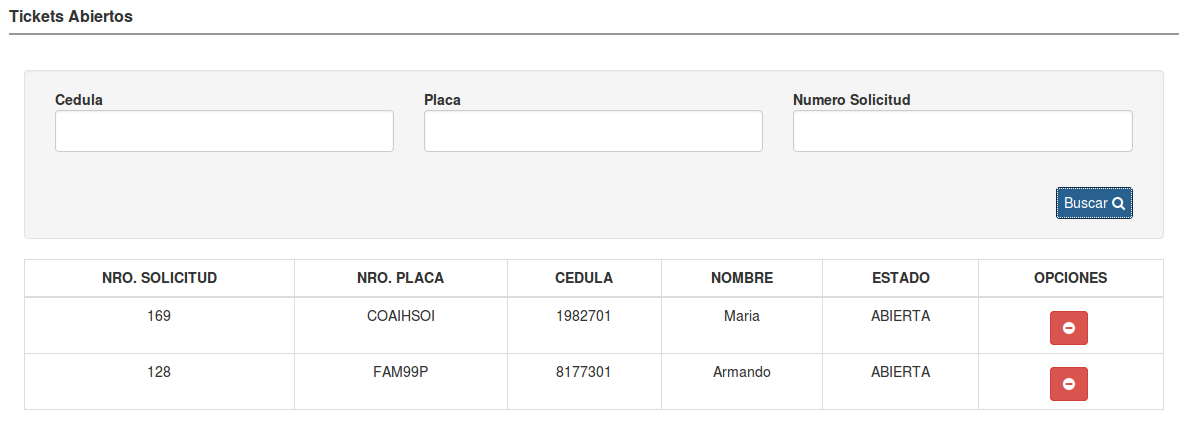
\includegraphics[width=\textwidth,height=7cm]{img/interfaces/bandeja_solicitudes_creadas.png}
\end{center}
\caption{Interfaz de bandeja solicitudes de inspección por Taquilla. Fuente: Print Screen.}
\label{fig:interfaz_bandeja_solicitudes_inspeccion_taquilla}
\end{figure}

En esta interfaz los usuarios taquilla pueden cancelar una solicitud de inspección siempre y cuando esta no este siendo atendida por algún inspector.



\textbf{-Modal eliminar solicitud de inspección}: La figura a continuación muestra el modal de confirmación para eliminar una solicitud de inspección.

\begin{figure}[H]
\begin{center}
	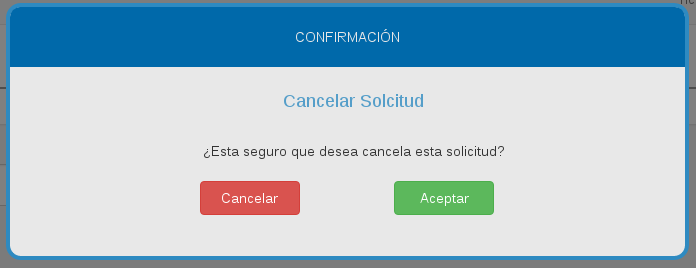
\includegraphics[width=14cm,height=6cm]{img/interfaces/modal_confirmacion_eliminar_solicitud_creada.png}
\end{center}
\caption{Modal eliminar solicitud de inspección. Fuente: Print Screen.}
\label{fig:modal_confirmacion_eliminar_solicitud}
\end{figure}


\textbf{-Interfaz Inspectores bandeja de solicitudes}: La figura a continuación muestra el filtro y bandeja de las solicitudes de inspección creadas.

\begin{figure}[H]
\begin{center}
	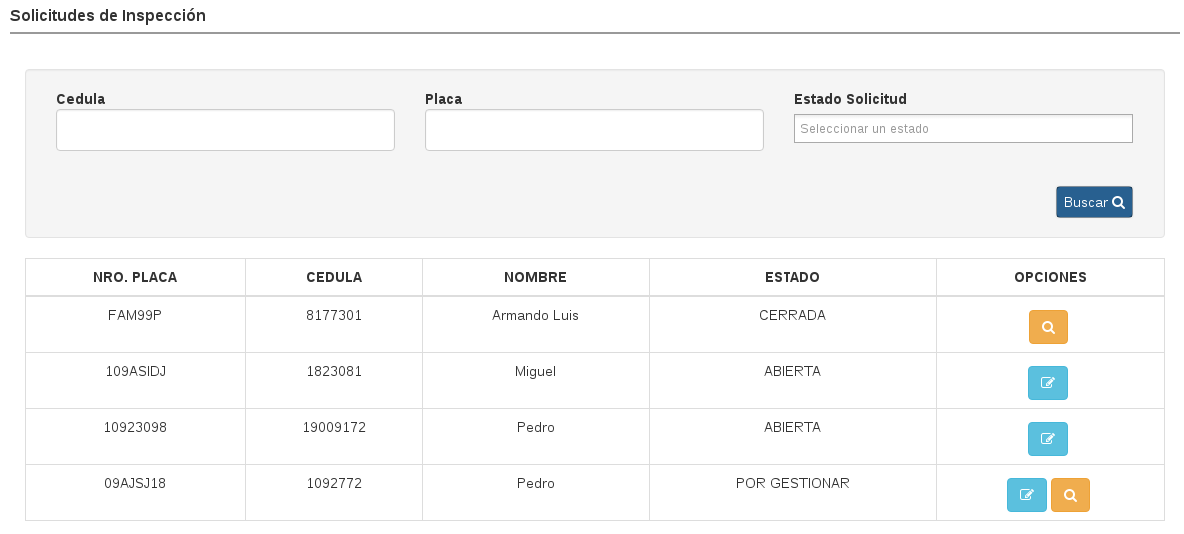
\includegraphics[width=\textwidth,height=7cm]{img/interfaces/bandeja_solicitudes_creadas_inspector.png}
\end{center}
\caption{Interfaz de bandeja solicitudes de inspección usuario Inspector. Fuente: Print Screen.}
\label{fig:interfaz_bandeja_solicitudes_inspeccion_inspector}
\end{figure}

En esta interfaz los usuarios inspector pueden registrar los datos de la inspección realizada, gestionar la solicitud de inspección y visualizar el documento generado por la solicitud.

\textbf{-Interfaz registro datos del vehículo en la solicitud de inspección}: La figura a continuación muestra el formulario para el registro de los datos del vehículo.

\begin{figure}[H]
\begin{center}
	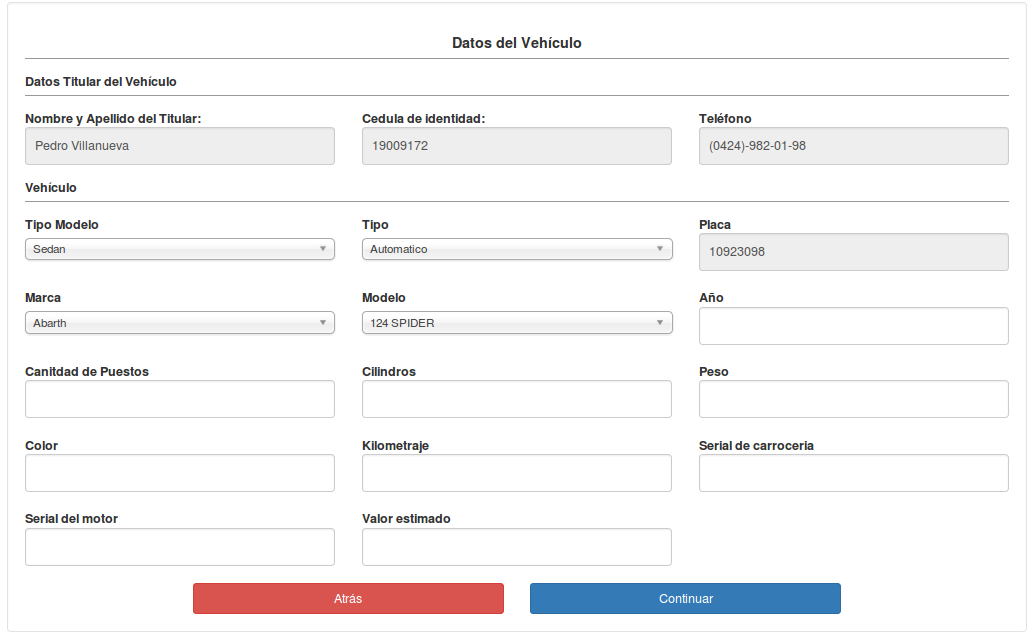
\includegraphics[width=\textwidth,height=7cm]{img/interfaces/registro_datos_vehiculo.png}
\end{center}
\caption{Interfaz del formulario de registro de los datos del vehículo. Fuente: Print Screen.}
\label{fig:interfaz_registro_datos_vehiculo}
\end{figure}

En esta interfaz los usuarios inspector pueden registrar los datos del vehículo de la inspección realizada. También dicha interfaz sirve para la gestión de la solicitud, mostrando los datos anteriormente cargados para su ultima revisión.

\newpage
\textbf{-Interfaz mecánica del vehículo en la solicitud de inspección}: La figura a continuación muestra el formulario para el registro de los datos de condiciones generales del vehículo.

\begin{figure}[H]
\begin{center}
	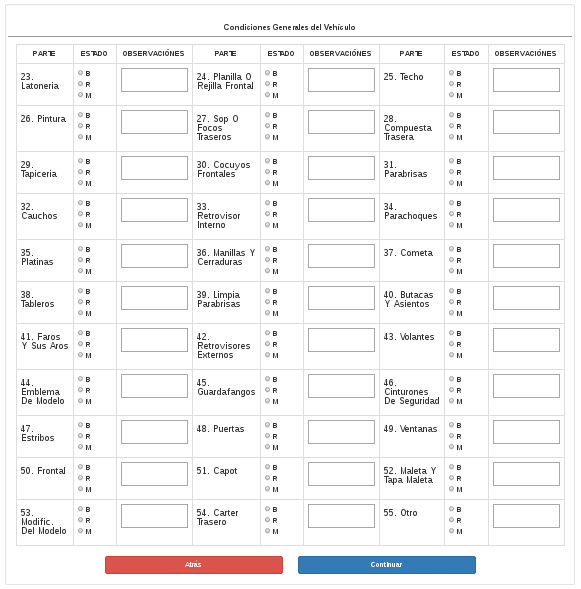
\includegraphics[width=\textwidth,height=16cm]{img/interfaces/registro_condiciones_generales_vehiculo.png}
\end{center}
\caption{Interfaz del formulario de registro de condiciones generales del vehículo. Fuente: Print Screen.}
\label{fig:interfaz_registro_condiciones_vehiculo}
\end{figure}

En esta interfaz los usuarios inspector pueden registrar los datos de las condiciones generales del vehículo de la inspección realizada. También dicha interfaz sirve para la gestión de la solicitud, mostrando los datos anteriormente cargados para su ultima revisión.


\textbf{-Interfaz mecánica del vehículo en la solicitud de inspección}: La figura a continuación muestra el formulario para el registro de los datos de la mecánica vehículo.

\begin{figure}[H]
\begin{center}
	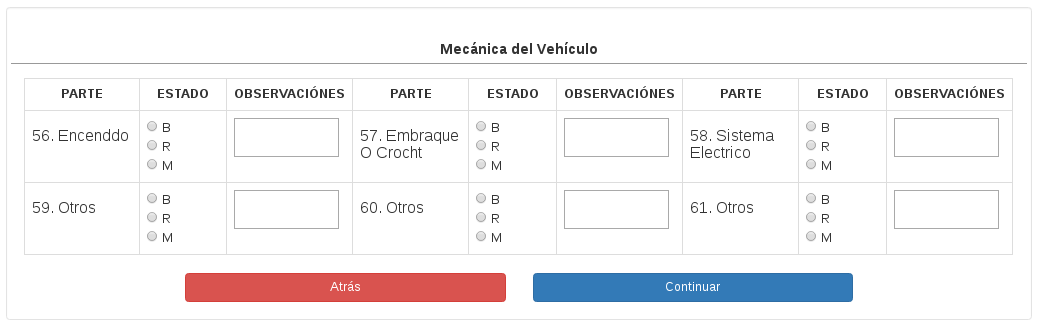
\includegraphics[width=\textwidth,height=6cm]{img/interfaces/registro_mecanica_vehiculo.png}
\end{center}
\caption{Interfaz del formulario de registro de la mecánica del vehículo. Fuente: Print Screen.}
\label{fig:interfaz_registro_mecanica_vehiculo}
\end{figure}

En esta interfaz los usuarios inspector pueden registrar los datos de la mecánica vehículo de la inspección realizada. También dicha interfaz sirve para la gestión de la solicitud, mostrando los datos anteriormente cargados para su ultima revisión.
\newpage
\textbf{-Interfaz accesorios del vehículo en la solicitud de inspección}: La figura a continuación muestra el formulario para el registro de los datos de los accesorios vehículo.

\begin{figure}[H]
\begin{center}
	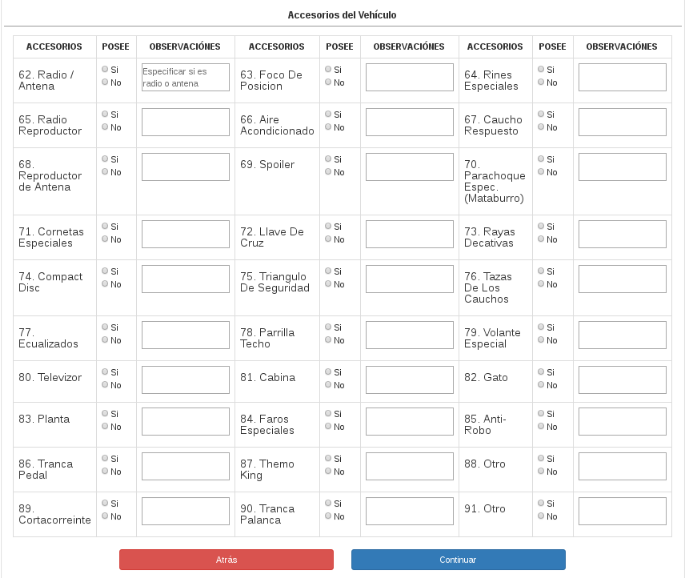
\includegraphics[width=\textwidth,height=16cm]{img/interfaces/registro_accesorios_vehiculo.png}
\end{center}
\caption{Interfaz del formulario de registro de los accesorios del vehículo. Fuente: Print Screen.}
\label{fig:interfaz_registro_accesorios_vehiculo}
\end{figure}

En esta interfaz los usuarios inspector pueden registrar los datos de los accesorios del vehículo de la inspección realizada. También dicha interfaz sirve para la gestión de la solicitud, mostrando los datos anteriormente cargados para su ultima revisión.


\textbf{-Interfaz detalles y datos del vehículo en la solicitud de inspección}: La figura a continuación muestra el formulario para el registro de los detalles y datos del vehículo.

\begin{figure}[H]
\begin{center}
	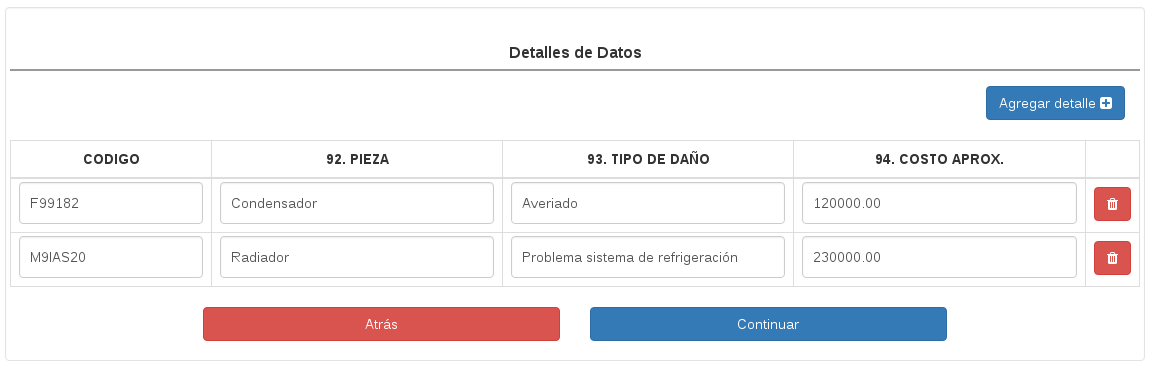
\includegraphics[width=\textwidth,height=6cm]{img/interfaces/registro_detalles_datos_vehiculo.png}
\end{center}
\caption{Interfaz del formulario de registro de los detalles y datos del vehículo. Fuente: Print Screen.}
\label{fig:interfaz_registro_detalles_datos_vehiculo}
\end{figure}

En esta interfaz los usuarios inspector pueden registrar los detalles y datos del vehículo de la inspección realizada. También dicha interfaz sirve para la gestión de la solicitud, mostrando los datos anteriormente cargados para su ultima revisión.

\textbf{-Interfaz documentos del vehículo en la solicitud de inspección}: La figura a continuación muestra el formulario para el registro de los documentos traídos del vehículo.

\begin{figure}[H]
\begin{center}
	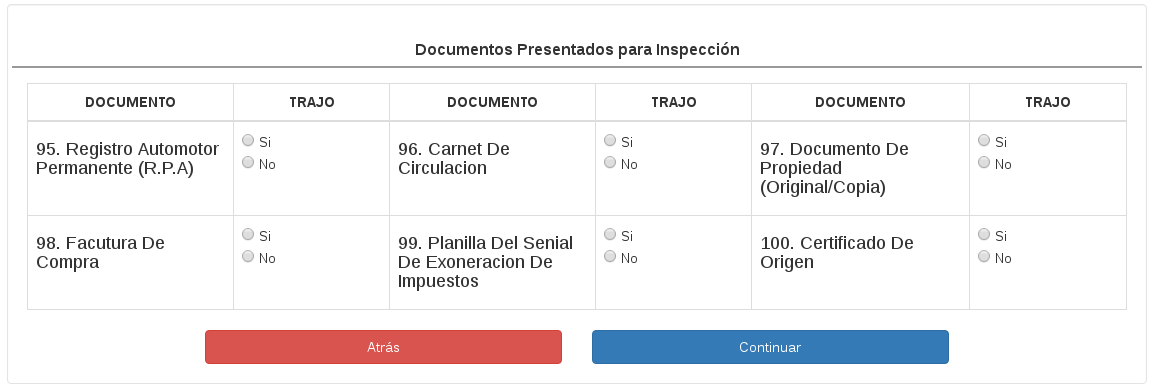
\includegraphics[width=\textwidth,height=6cm]{img/interfaces/registro_documentos_presentados_vehiculo.png}
\end{center}
\caption{Interfaz del formulario de registro de los documentos del vehículo. Fuente: Print Screen.}
\label{fig:interfaz_registro_documentos_vehiculo}
\end{figure}

En esta interfaz los usuarios inspector pueden registrar los documentos que trajeron del vehículo de la inspección realizada. También dicha interfaz sirve para la gestión de la solicitud, mostrando los datos anteriormente cargados para su ultima revisión.

\newpage
\textbf{-Interfaz vista previa de la solicitud de inspección}: La figura a continuación muestra el formulario para el registro de las observaciones referente a la inspección del vehículo y una vista previa de como quedara la solicitud.

\begin{figure}[H]
\begin{center}
	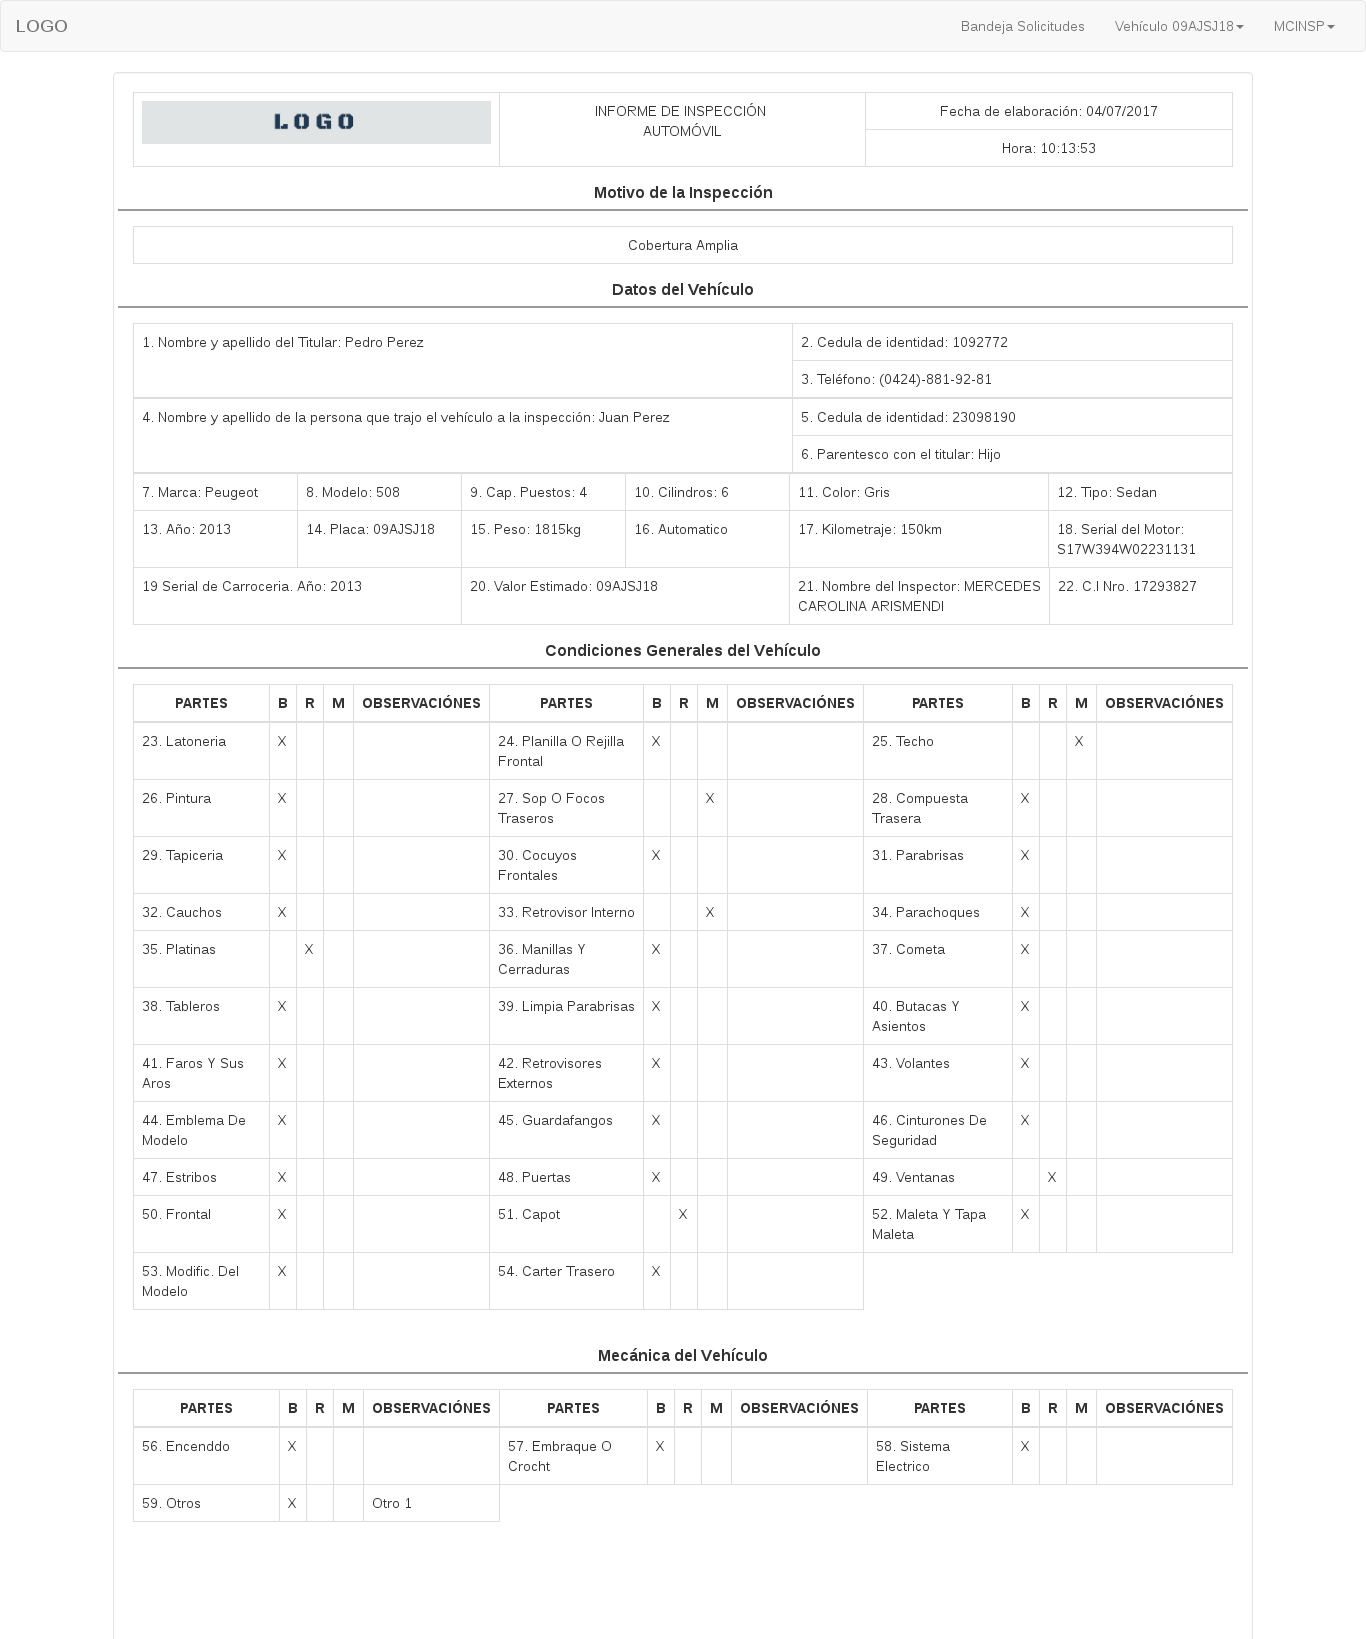
\includegraphics[width=\textwidth,height=18cm]{img/interfaces/prev_planilla_1.png}
\end{center}
\caption{Interfaz de la vista previa de los datos del vehículo (Parte 1). Fuente: Print Screen.}
\label{fig:interfaz_vista_previa_vehiculo_1}
\end{figure}

\begin{figure}[H]
\begin{center}
	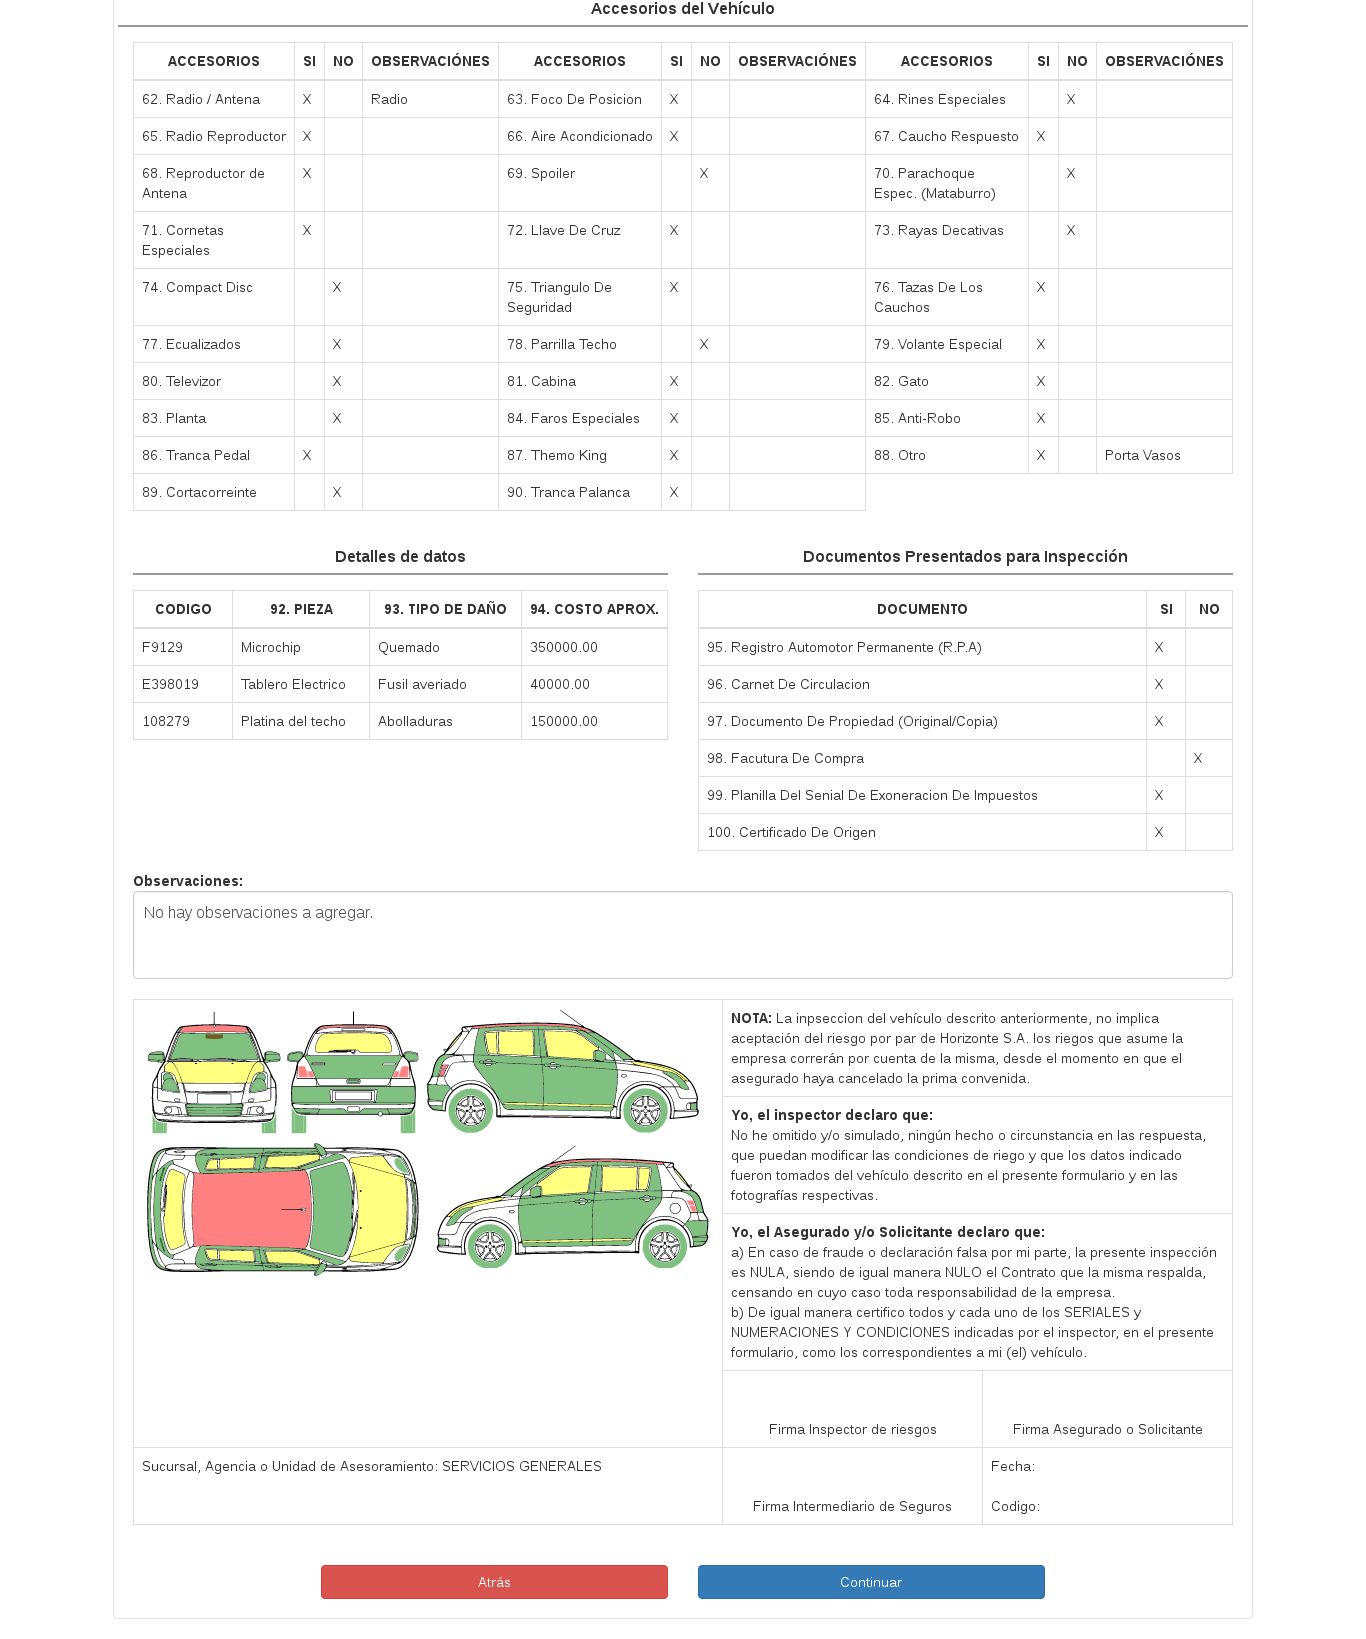
\includegraphics[width=\textwidth,height=19cm]{img/interfaces/prev_planilla_2.png}
\end{center}
\caption{Interfaz de la vista previa de los datos del vehículo (Parte 2). Fuente: Print Screen.}
\label{fig:interfaz_vista_previa_vehiculo_2}
\end{figure}

En esta interfaz los usuarios inspector pueden verificar todo los datos del vehículo de la inspección realizada. También dicha interfaz sirve para la gestión de la solicitud, mostrando los datos anteriormente cargados para su ultima revisión.


\textbf{-Modal finalizar registro de inspección}: La figura a continuación muestra el modal de confirmación para registrar los datos de una solicitud de inspección.

\begin{figure}[H]
\begin{center}
	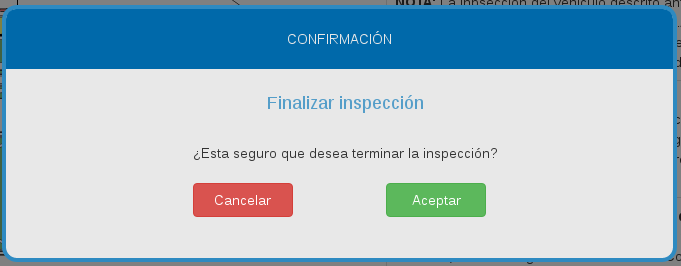
\includegraphics[width=14cm,height=6cm]{img/interfaces/modal_finalizar_inspeccion.png}
\end{center}
\caption{Modal finalizar la solicitud de inspección. Fuente: Print Screen.}
\label{fig:modal_finalizar_registro_dato_solicitud}
\end{figure}

\setlength{\parskip}{0mm}



\textbf{-Modal finalizar gestión de inspección}: La figura a continuación muestra el modal de confirmación para finalizar la solicitud de inspección de manera definitiva.

\begin{figure}[H]
\begin{center}
	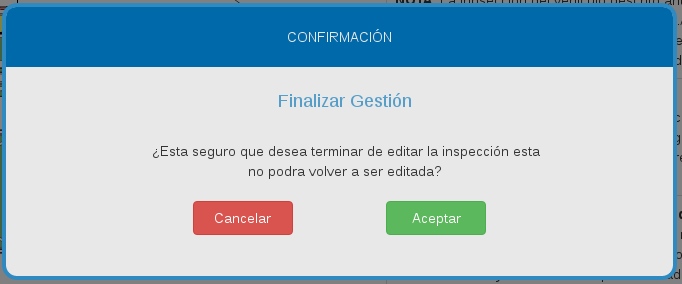
\includegraphics[width=14cm,height=6cm]{img/interfaces/modal_finalizar_gestion.png}
\end{center}
\caption{Modal finalizar la solicitud de inspección. Fuente: Print Screen.}
\label{fig:modal_finalizar_gestion_dato_solicitud}
\end{figure}

\setlength{\parskip}{0mm}




\section{Fase de pruebas } 
\setlength{\parskip}{5mm}
Las pruebas realizadas para verificar el correcto funcionamiento del sistema y la aceptación de los usuarios por el mismo se dividieron en dos (2) partes a continuación se explica detalladamente las mismas.

\setlength{\parskip}{0mm}



\subsection{Pruebas funcionales}
\setlength{\parskip}{5mm}


Para estas pruebas se realizo una tabla mostrada a continuación, en la cual se especifican los módulos pertenecientes al sistema y las funcionalidades que debería tener cada uno de ellos, estas fueron probadas por usuarios especialmente seleccionados que poseyeran un criterio de evaluación acertijo y critico en cuanto a los resultados. 
\setlength{\parskip}{0mm}

\begin{table}[H]	
\begin{center}
\begin{tabular}{ | m{4cm} | m{8cm}| m{3cm}| } 
 \hline
 Modulo & Funcionalidades Probadas & Resultados \\
 \hline
 Administración. 
 & 
 \begin{itemize}
 	\item Modificacion de Usuarios.
 	\item Modificacion de Clientes.
 \end{itemize}. 
 & 
 .\\

 \hline
 Registro. 
 & 
 \begin{itemize}
 	\item Registrar cuenta
 \end{itemize}. 
 & 
 .\\

 \hline
 Perfil. 
 & 
 \begin{itemize}
 	\item Editar información del usuario
 \end{itemize}. 
 & 
 .\\

 \hline
 
 Recuperar Contraseña.
 & 
 \begin{itemize}
 	\item Recuperar Contraseña 
 \end{itemize}. 
 & 
 .\\

 \hline

 \end{tabular}
\caption{Instrumento evaluación módulos del sistema (Parte 1). Fuente: El autor}
\label{Tabla:7}
\end{center}
\end{table}	

\newpage

\begin{table}[H]	
\begin{center}
\begin{tabular}{ | m{4cm} | m{8cm}| m{3cm}| } 
 \hline
 Modulo & Funcionalidades Probadas & Resultados \\
 \hline
 

 Consulta. 
 & 
 \begin{itemize}
 	\item Consultar solicitudes creadas.
 	\item Consultar Usuarios de la aplicación.
 	\item Consultar titulares de carros.
 	\item Consultar personas que trajeron el vehículo a la inspección. 
 \end{itemize}. 
 & 
 .\\

  \hline
 Solicitud. 
 & 
 \begin{itemize}
 	\item Realizar solicitud de inspección
 \end{itemize}. 
 & 
 .\\

 \hline
 Gestión de Solicitudes. 
 & 
 \begin{itemize}
 	\item Registrar los datos de la solicitud de inspección
 	\item Gestionar la solicitud de inspección
 \end{itemize}. 
 & 
 .\\

 \hline
\end{tabular}
\caption{Instrumento evaluación módulos del sistema (Parte 2). Fuente: El autor}
\label{Tabla:7}
\end{center}
\end{table}	

\setlength{\parskip}{5mm}

\newpage
Las pruebas presentadas en esta tabla se fueron realizando mediante ciclos hasta lograr la completa aprobación de lo módulos.

\begin{table}[H]	
\begin{center}
\begin{tabular}{ | m{2cm} | m{4.5cm} | m{4.5cm}| m{4.5cm}| } 
 \hline
  & \multicolumn{3}{|c|}{Ciclo de Prueba}  \\
 \hline
 Usuario. & 1. & 2. & 3.\\
 \hline
 1. 
 & 
 \begin{itemize}
 	\item 3 módulos aprobados
 	\item 4 módulos no aprobados
 \end{itemize}. 
 & 
 \begin{itemize}
 	\item 5 módulos aprobados
 	\item 2 módulos no aprobados
 \end{itemize}.
 & 
 \begin{itemize}
 	\item 7 módulos aprobados.
 \end{itemize}.\\
 \hline
 2. 
 & 
 \begin{itemize}
 	\item 3 módulos aprobados
 	\item 4 módulos no aprobados
 \end{itemize}. 
 & 
 \begin{itemize}
 	\item 5 módulos aprobados
 	\item 2 módulos no aprobados
 \end{itemize}.
 & 
 \begin{itemize}
 	\item 7 módulos aprobados.
 \end{itemize}.\\
 \hline
 3. 
 & 
 \begin{itemize}
 	\item 3 módulos aprobados
 	\item 4 módulos no aprobados
 \end{itemize}. 
 & 
 \begin{itemize}
 	\item 5 módulos aprobados
 	\item 2 módulos no aprobados
 \end{itemize}.
 & 
 \begin{itemize}
 	\item 7 módulos aprobados.
 \end{itemize}.\\
 \hline
\end{tabular}
\caption{Matriz de ciclos de pruebas. Fuente: El autor}
\label{Tabla:7}
\end{center}
\end{table}


\textbf{-Ciclo 1}: 
\begin{itemize}
	\item Usuario 1: de los 7 módulos probados, 4 terminaron con el estatus de no aprobación. Las funcionalidades que fallaron fueron las siguientes:
	 \begin{itemize}
			\item  El correo no se enviaba correctamente a los usuarios registrados.
			\item  Campos numéricos aceptaban caracteres.
			\item  Datos de las solicitudes de inspección siempre se precargaban los mismos, y cuando se cambia en algún cliente se cambian en todos.
			\item  Inactivar usuarios.
		  \end{itemize}

	\item Usuario 2: de los 7 módulos probados, 4 terminaron con el estatus de no aprobación. Las funcionalidades que fallaron fueron las siguientes:
	 \begin{itemize}
			\item  El correo no se enviaba correctamente a los usuarios registrados.
			\item  Campos numéricos aceptaban caracteres.
			\item  Inactivar usuarios.
			\item  Datos inconsistentes en diferentes solicitudes de inspección.
		  \end{itemize}

	\item Usuario 3: de los 7 módulos probados, 4 terminaron con el estatus de no aprobación. Las funcionalidades que fallaron fueron las siguientes:
	 \begin{itemize}
			\item  No llega el correo al registrar el usuario
			\item  Error en montos al colocar carácter.
			\item  Datos de las solicitudes de inspección siempre se precargaban los mismos, y cuando se cambia en algún cliente se cambian en todos.
			\item  Inactivar usuarios.
		  \end{itemize}

\end{itemize}

\textbf{-Ciclo 2}: 
\begin{itemize}
	\item Usuario 1: de los 7 módulos probados, 2 terminaron con el estatus de no aprobación. Las funcionalidades que fallaron fueron las siguientes:
	 \begin{itemize}
			\item Consultar titulares del vehículo no funcionaba consultar por numero.
			\item Consultar titulares del vehículo no funcionaba consultar por numero.
			\item Al terminar la solicitud de inspección, no se muestra en el pdf las observaciones realizadas
		  \end{itemize}

	\item Usuario 2: de los 7 módulos probados, 2 terminaron con el estatus de no aprobación. Las funcionalidades que fallaron fueron las siguientes:
	 \begin{itemize}
	 		\item Consultar titulares del vehículo no funcionaba consultar por numero.
			\item Consultar titulares del vehículo no funcionaba consultar por numero.
			\item Al terminar la solicitud de inspección, no se muestra en el pdf las observaciones realizadas
		  \end{itemize}

	\item Usuario 3: de los 7 módulos probados, 2 terminaron con el estatus de no aprobación. Las funcionalidades que fallaron fueron las siguientes:
	 \begin{itemize}
			\item Consultar titulares del vehículo no funcionaba consultar por numero.
			\item Consultar titulares del vehículo no funcionaba consultar por numero.
			\item Al terminar la solicitud de inspección, no se muestra en el pdf las observaciones realizadas
		  \end{itemize}

\end{itemize}

\textbf{-Ciclo 3}: En este ciclo todos los usuarios aprobaron todas las funcionalidades del sistema de todos los módulos.

\setlength{\parskip}{0mm}

\subsection{Pruebas de aceptación}
\setlength{\parskip}{5mm}

Para comprobar el nivel de aceptación del sistema, se realizo una encuesta correspondiente a las interfaces del sistema orientadas a la usabilidad. Dicha encuesta fue realizada a un grupo de diez personas. De esta manera se pudo obtener un feed back de parte de los usuarios para mejorar las interfaces del sistema.



\begin{table}[H]	
\begin{center}
\begin{tabular}{ | m{1cm} | m{8cm}| m{1cm}|m{1cm}| m{1cm} | m{1cm}| m{1cm}| } 
 \hline
 \multicolumn{2}{|c|}{} & 1 & 2 & 3 & 4 & 5 \\
 \hline
 1 & La aplicación es intuitiva & & & & & \\
 \hline
 2 & Considera usted que los colores crean un buen contraste. & & & & & \\
 \hline
 3 & El diseño y estilo de la aplicación es consistente a lo largo de sus interfaces & & & & & \\
 \hline
 4 & El lenguaje usado en la aplicación es claro & & & & & \\
 \hline
 5 & La aplicación ofrece mensajes acordes a las operaciones realizadas. & & & & & \\
 \hline
 6 & Es posible navegar por la aplicación sin perderse & & & & & \\
 \hline
 7 & La aplicación es usable & & & & & \\
 \hline
 8 & Las acciones realizadas son fáciles de memorizar & & & & & \\
 \hline
 9 & La aplicación muestra mensajes de errores explícitos de acuerdo al error ocurrido & & & & & \\
 \hline
\end{tabular}
\caption{Encuesta de aceptación. Fuente: El Autor}
\label{Tabla:8}
\end{center}
\end{table}	


Para el desarrollo de esta encuesta se deben seleccionar valores que van desde "Totalmente en desacuerdo" hasta "Totalmente de acuerdo", estableciendo un rango de numero del 1 al 5.

Los resultados de las encuestas aplicadas, para evaluar el nivel de aceptación, se pueden apreciar en las siguientes Figuras.

\newpage
\textbf{-Resultado de las encuestas}: 


\begin{figure}[H]
\begin{center}
	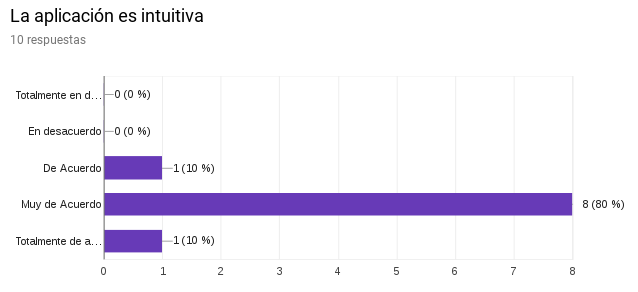
\includegraphics[width=\textwidth,height=7cm]{img/encuestas/aplicacion_intuitiva.png}
\end{center}
\caption{Resultados de la pregunta 1. Fuente: El Autor.}
\label{fig:respuesta_aplicacion_intuitiva}
\end{figure}


\begin{figure}[H]
\begin{center}
	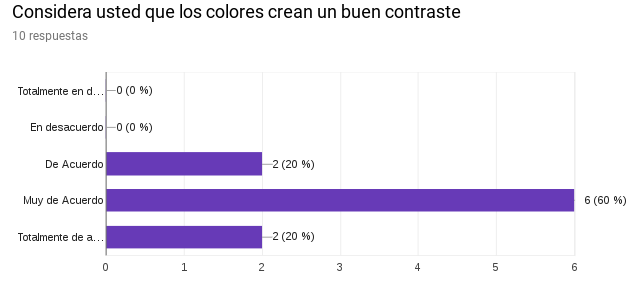
\includegraphics[width=\textwidth,height=7cm]{img/encuestas/contraste_colores.png}
\end{center}
\caption{Resultados de la pregunta 2. Fuente: El Autor.}
\label{fig:respuesta_contraste_colores}
\end{figure}

\newpage

\begin{figure}[H]
\begin{center}
	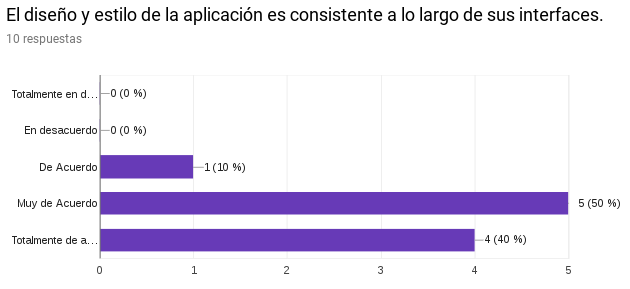
\includegraphics[width=\textwidth,height=7cm]{img/encuestas/diseno_consistente.png}
\end{center}
\caption{Resultados de la pregunta 3. Fuente: El Autor.}
\label{fig:respuesta_diseno_consistente}
\end{figure}

\begin{figure}[H]
\begin{center}
	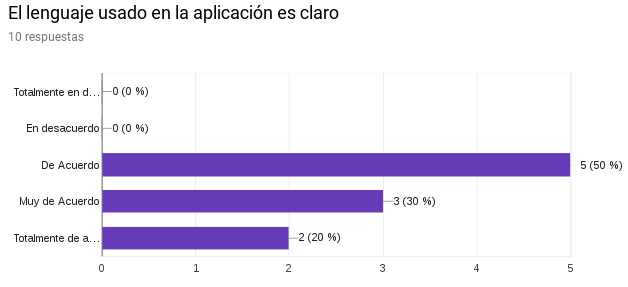
\includegraphics[width=\textwidth,height=7cm]{img/encuestas/lenguaje_usado.png}
\end{center}
\caption{Resultados de la pregunta 4. Fuente: El Autor.}
\label{fig:respuesta_lenguaje_usado}
\end{figure}



\newpage
\begin{figure}[H]
\begin{center}
	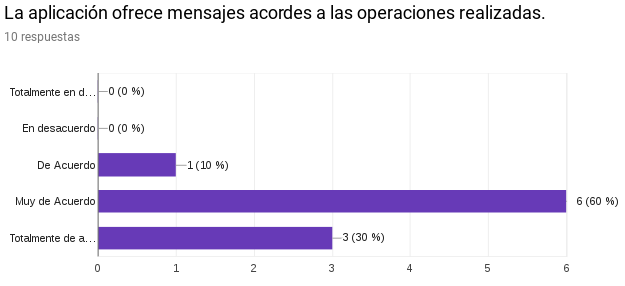
\includegraphics[width=\textwidth,height=7cm]{img/encuestas/mensajes_acordes.png}
\end{center}
\caption{Resultados de la pregunta 5. Fuente: El Autor.}
\label{fig:respuesta_mensajes_acordes}
\end{figure}

\begin{figure}[H]
\begin{center}
	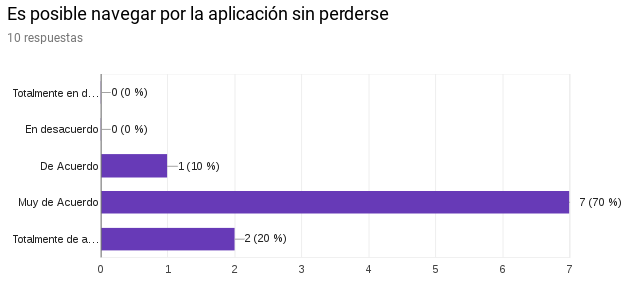
\includegraphics[width=\textwidth,height=7cm]{img/encuestas/navegar_sin_perdida.png}
\end{center}
\caption{Resultados de la pregunta 6. Fuente: El Autor.}
\label{fig:respuesta_navegar_sin_perdida}
\end{figure}
\newpage
\begin{figure}[H]
\begin{center}
	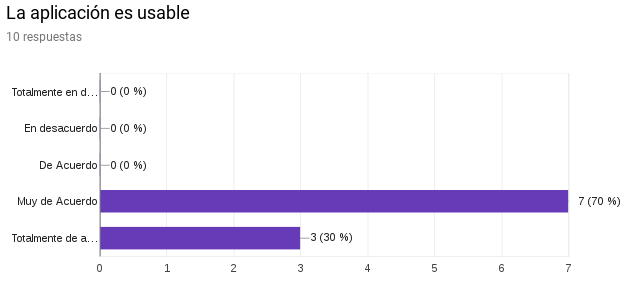
\includegraphics[width=\textwidth,height=7cm]{img/encuestas/aplicacion_usable.png}
\end{center}
\caption{Resultados de la pregunta 7. Fuente: El Autor.}
\label{fig:respuesta_aplicacion_usable}
\end{figure}

\begin{figure}[H]
\begin{center}
	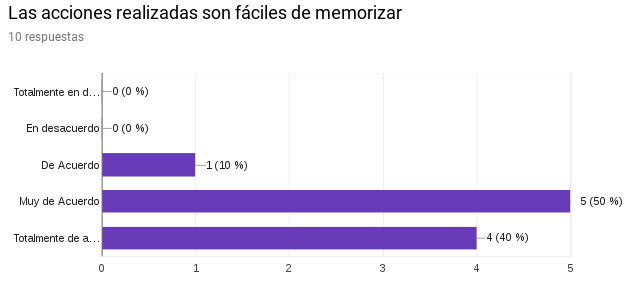
\includegraphics[width=\textwidth,height=7cm]{img/encuestas/acciones_memorizables.png}
\end{center}
\caption{Resultados de la pregunta 8. Fuente: El Autor.}
\label{fig:respuesta_acciones_memorizables}
\end{figure}
\newpage
\begin{figure}[H]
\begin{center}
	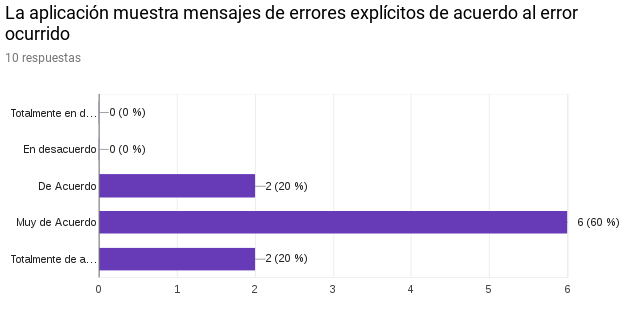
\includegraphics[width=\textwidth,height=7cm]{img/encuestas/mensajes_errores_explicitos.png}
\end{center}
\caption{Resultados de la pregunta 9. Fuente: El Autor.}
\label{fig:respuesta_mensajes_errores_explicitos}
\end{figure}

Con base a los resultados anteriores se puede concluir que la aplicación es bastante intuitiva, utiliza colores que crean buen contraste y haciendo la aplicación consistente entre sus interfaces, logrando así gran usabilidad. Además se puede apreciar que el lenguaje utilizado en la aplicación tanto como los mensajes de respuesta de la misma son de agrado para los usuarios aunque en parte del lenguaje de la aplicación hay ciertos tecnicismos los cuales le dan un nivel de complejidad a los mismos. Aun así por ser intuitiva, es fácil recordar las acciones realizadas.


\setlength{\parskip}{0mm}

